\documentclass[a4paper,fleqn,titlepage,11pt]{article}
\usepackage{t1enc} 
%%\usepackage{german}

%%\selectlanguage{german}


\pagestyle{myheadings}
\pagenumbering{arabic}
\setlength{\parindent}{0mm}		% Einzug f�r die erste Zeile im Absatz

%% Seitenformat:
\setlength{\oddsidemargin}{0cm}		% li. Randabstand auf re. Seiten
\setlength{\textwidth}{16cm}		% Breite des Textes
\setlength{\topmargin}{-0.75cm}		% Abst. Oberkante Blatt - Oberk. Header
\setlength{\headheight}{30pt}		% H�he des Headers
\setlength{\headsep}{5mm}		% Abst. Header - Text
\setlength{\topskip}{5mm}		% Oberkante Text - Grundlinie 1. Z.
\setlength{\textheight}{23.5cm}		% H�he des Textes
%%\setlength{\footheight}{0cm}		% H�he des Footers
\setlength{\footskip}{1cm}		% Abst. Unterk. Text - Unterk. Footer

\usepackage{graphicx}

\begin{document}

\thispagestyle{empty}

\begin{center}
\LARGE
Workshop Guide

\vspace{1cm}

Restructuring Code: From ``Push''  To ``Pull''
\end{center}

\normalsize

\vspace{0.6cm}

%%%%%%%%%%%%%%%%%%%%%%%%%%%%%%%%%%%%%%%%%%%%%%%%%%

\section*{Overview}

\subsection*{The Initial Situation}

The restructuring pattern ``From Push to Pull'' is applicable to code that follows the general pattern described here.

\subsubsection*{Goal of the Code}

The code produces a sequence of data objects, each of which may hold several data (e.g.~several numbers).

\subsubsection*{Shape of the Code}

The general structure of the code is similar to this:

\begin{itemize}
\item one class for a single input data (here: the class \texttt{Transaction})
\item a sequence of these input data elements (here: \texttt{List<Transaction>})
\item very few classes with logic (here: the class \texttt{PushingBalancesCalculator})
\item one class for a single output data entry (here: \texttt{BalancesOfMonth})
\item a sequence of these output data elements (here: \texttt{List<BalancesOfMonth>}) which is constructed early in the program run
\end{itemize}

The basic mechanics of the logic class(es) is as follows:

\begin{itemize}
\item initially, the sequence of output data is not filled
\item the main logic part consists of two interlaced loops: 
\begin{itemize}
\item the outer loop iterates over the sequence of output data objects (here: the months for which the output data is to be determined)
\item the inner loop iterates over the sequence of input data objects and calculates the data for one output data object (here: the sum of the transactions for each month)
\item at the end of the inner loop, the calculated data is written to that output data object (``push'')
\end{itemize}
\item finally, the sequence of output data is filled
\item the logic class(es) may contain multiple of these interlaced loops in sequence, where a subsequent loop may access and modify the output data that a previous loop has calculated and pushed to the sequence of output data
\end{itemize}

\subsubsection*{First Impressions of the Code}
The code doesn't look too bad. It has some issues. The algorithm is not easy to understand. Testing is only possible on an integration base. There is no isolation or abstraction.

\subsection*{Desired Final Situation}

The code should be crisper. That means: easy to read, understand, test and extend.

The overall goal is to extract the calculations of the individual values into separate methods.

This can be broken up into three major parts:

\begin{enumerate}
\item Disentangle the for loops, isolate the loop body and extract it
\item Build one data object for each loop iteration (instead of reusing the same object over and over again)
\item Isolate the calculations of the distinct values into separate methods and calculate them on demand
\end{enumerate}

In the following, we will split up these two parts into fine-grained steps that can be applied to the code.

We do this by:
\begin{itemize}
	\item Defining one interaction point with outside objects (Step 1)
	\item Separating value calculation from iteration (Steps 2-4)
	\item Encapsulating the calculation object (Steps 5-6)
	\item Separating calculation for each value (Step 7-8)
	\item Eliminating unwanted state (Step 9-10)
	\item Tidying up (Step 11)
	\item Achieving the ``Pull'' Structure (Final Step)
\end{itemize}

\subsubsection*{Restrictions / Rules:}


\begin{itemize}
\item Change one thing at a time.

\item Right now, we neither want to change the outside world nor our calculator class API, only the internals of our calculator class. The result objects (\texttt{BalancesOfMonth}) represent the outside world in our example. Therefore, we will leave the result objects and the \texttt{fillData} method signature untouched. 
\end{itemize}


\textbf{Note:} The workspace with the step number contains the \textbf{solution} to the step!

\section*{Part I: Disentangle the For Loops and Extract the Loop Body}

\subsubsection*{Overall Goal:}

Extract most of the outer for loop body into a separate method. This new method must not know about the result object!

\subsection*{Pre-Arrangements (Workspace: Push)}

Tidy up the code, rename local variables to make their names more descriptive.
Push the loops as far to the outside of the method as possible (move as much code as possible inside the loop bodies).

\subsection*{Step 01: Decoupling from the outside world}

\subsubsection*{Observations:}
\begin{itemize}
\item The outer loop iterates over the list of result objects that need to be filled with the calculated data.
\item The method calculates two values for each result object: \texttt{balance} and \texttt{averageBalance}. 
\item These two values cannot both be returned from a single method.
\end{itemize}

\subsubsection*{Solution:}

Create an object that will transport the calculated values. 
This intermediate object will only hold the values, it will not contain any logic. It will have one setter that sets all calculated values simultaneously. It will also have getters, one for each of the calculated values.

In the main logic part, we will create one such intermediate object at the beginning of the calculation. Instead of directly writing the calculated values to the output data structure, we write them to the intermediate object and then read them again from the intermediate object in order to write them to the output data structure. We reuse the same intermediate object for each run through the loop.

\subsubsection*{Modified:}

\texttt{ValuesOfMonth} is created

\texttt{PushingBalancesCalculator.fillData()}

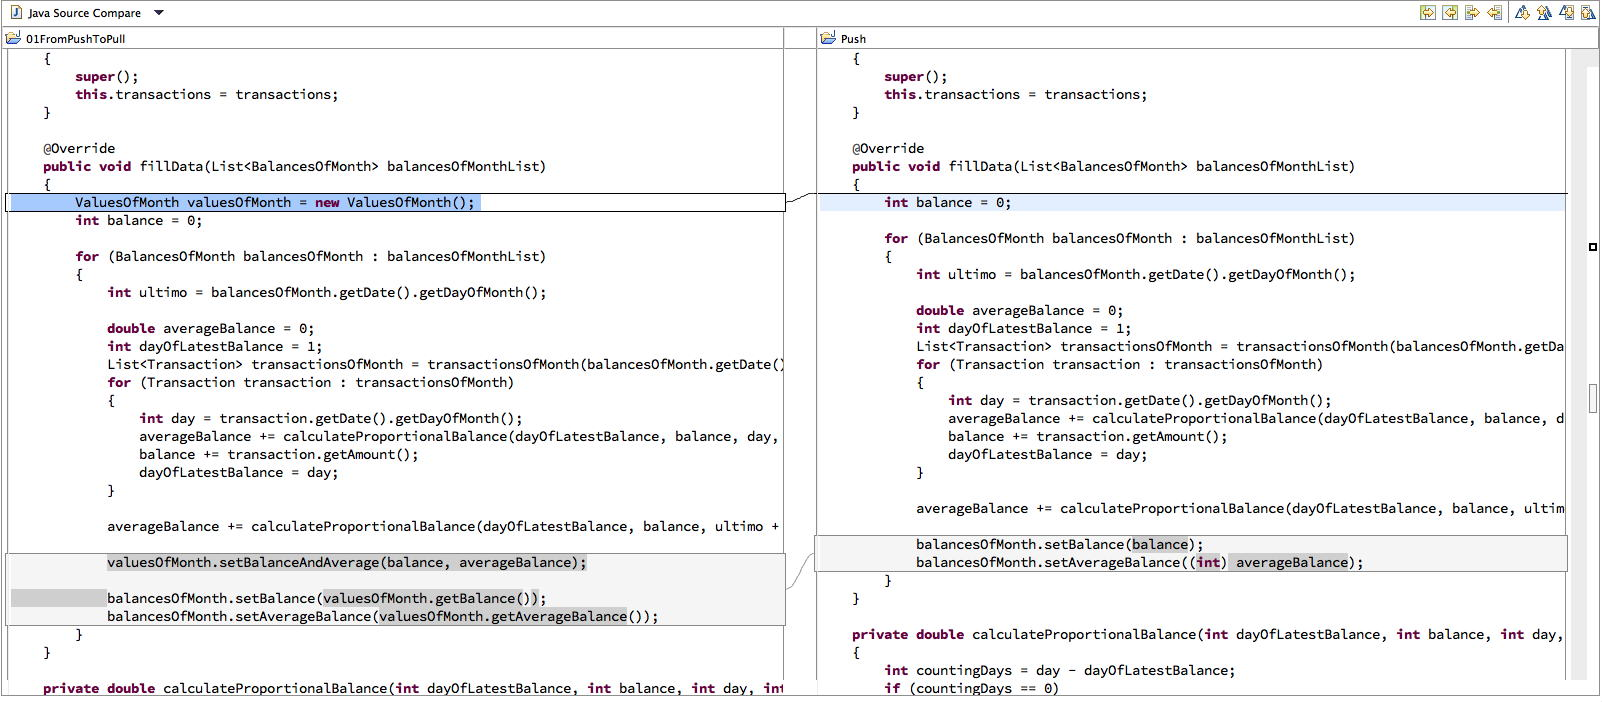
\includegraphics[width=1\textwidth]{CompareViews/Push-01.jpg}


\subsection*{Step 02: Preparing for method extraction: Purifying the dependencies}

\subsubsection*{Observations:}
\begin{itemize}
\item We only need the date from the \texttt{BalancesOfMonth} object, namely for calculating the current ultimo.
\item If we extracted the body of the outer loop into a method, this method would depend on our outer world, i.e. \texttt{BalancesOfMonth}.
\item If we extracted the body of the outer loop into a method, this method would depend on state of our object, namely \texttt{transactions} (inside \texttt{transactionsOfMonth}).
\end{itemize}

Both dependencies are undesirable.

\subsubsection*{Solution:}

\begin{itemize}
\item Move the transaction filtering to the top of the loop.
\item Extract the date from the \texttt{BalancesOfMonth} object, move it to the top of the loop and use it in the rest of the method body.
\end{itemize}

\subsubsection*{Modified:}

\texttt{PushingBalancesCalculator.fillData()}

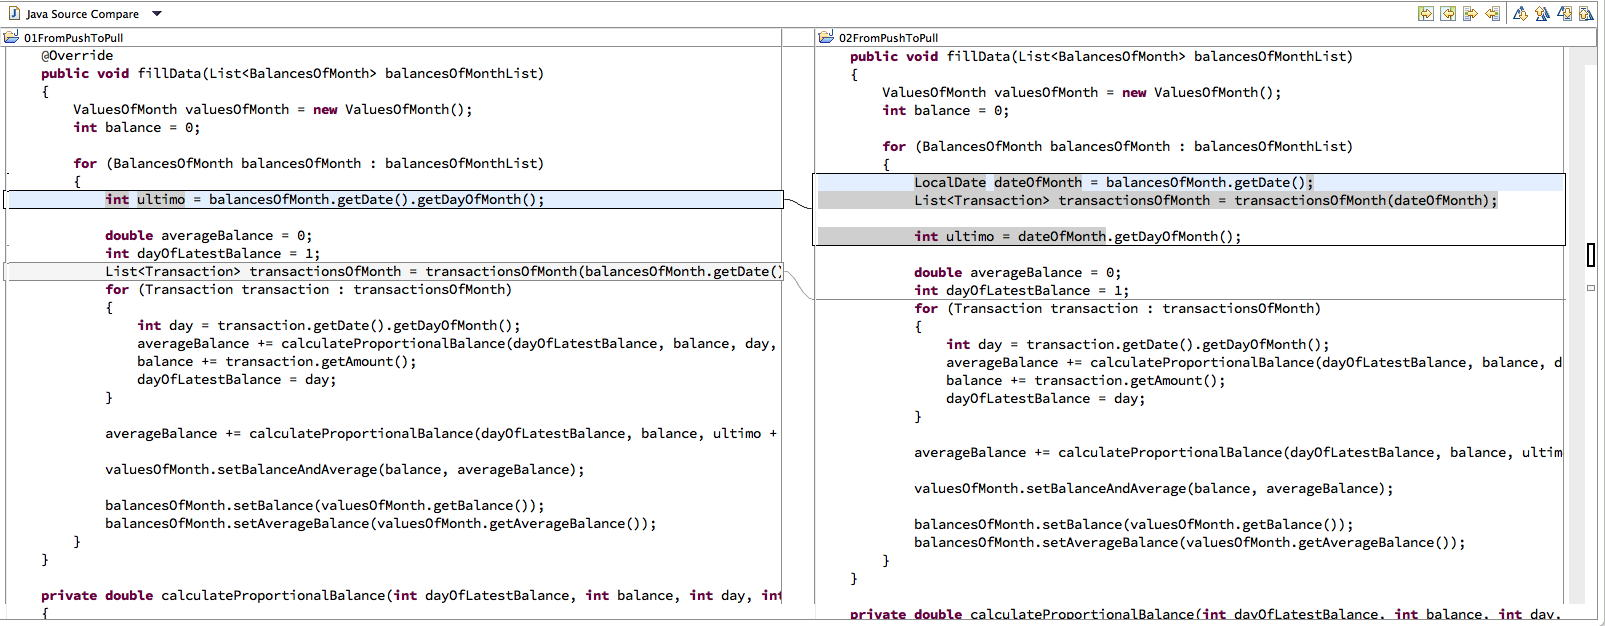
\includegraphics[width=1\textwidth]{CompareViews/01-02.jpg}


\subsection*{Step 03: Separation of Calculation and Iteration}

\subsubsection*{Observations:}
\begin{itemize}
\item We can now extract the major part of the method body into a separate method.
\end{itemize}

\subsubsection*{Solution:}

Let's do it!

\subsubsection*{Modified:}

\texttt{PushingBalancesCalculator.fillData()}

\texttt{PushingBalancesCalculator.calculateValuesForMonth()} is created

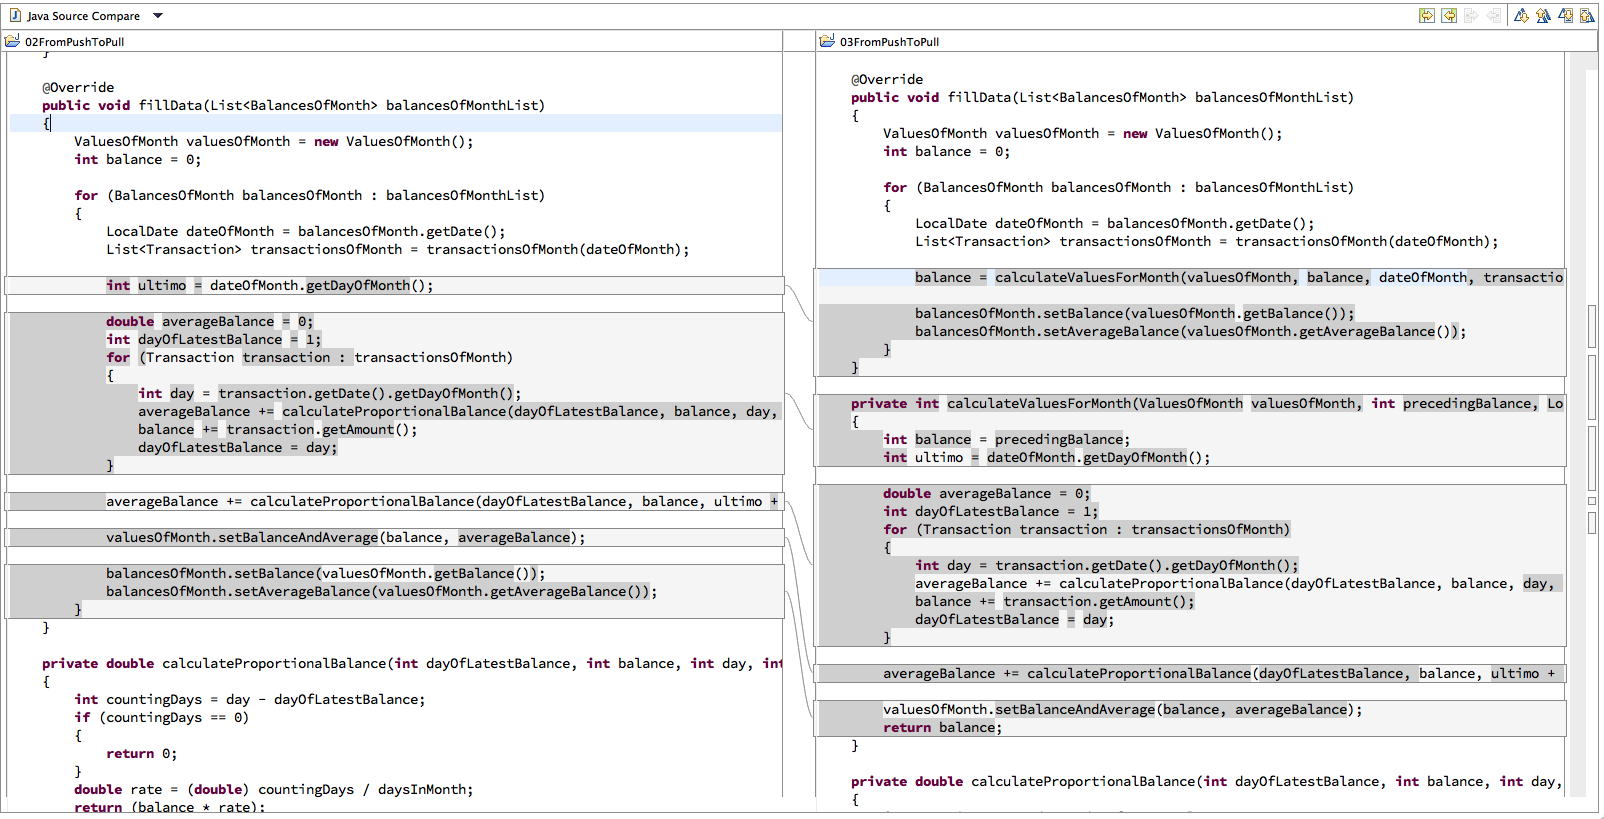
\includegraphics[width=1\textwidth]{CompareViews/02-03.jpg}



\section*{Part II: One object for each loop iteration}

\subsubsection*{Overall Goal:}

Build one data object for each loop iteration (instead of reusing the same object over and over again).


\subsection*{Step 04: Turn out-parameter into returned value}

\subsubsection*{Observations:}
\begin{itemize}
\item The first parameter in \texttt{calculateValuesForMonth()} acts as in/out parameter.
\end{itemize}

\subsubsection*{Solution:}
Create an explicit return object and delete this parameter.

\subsubsection*{Modified:}

\texttt{PushingBalancesCalculator.calculateValuesForMonth()}

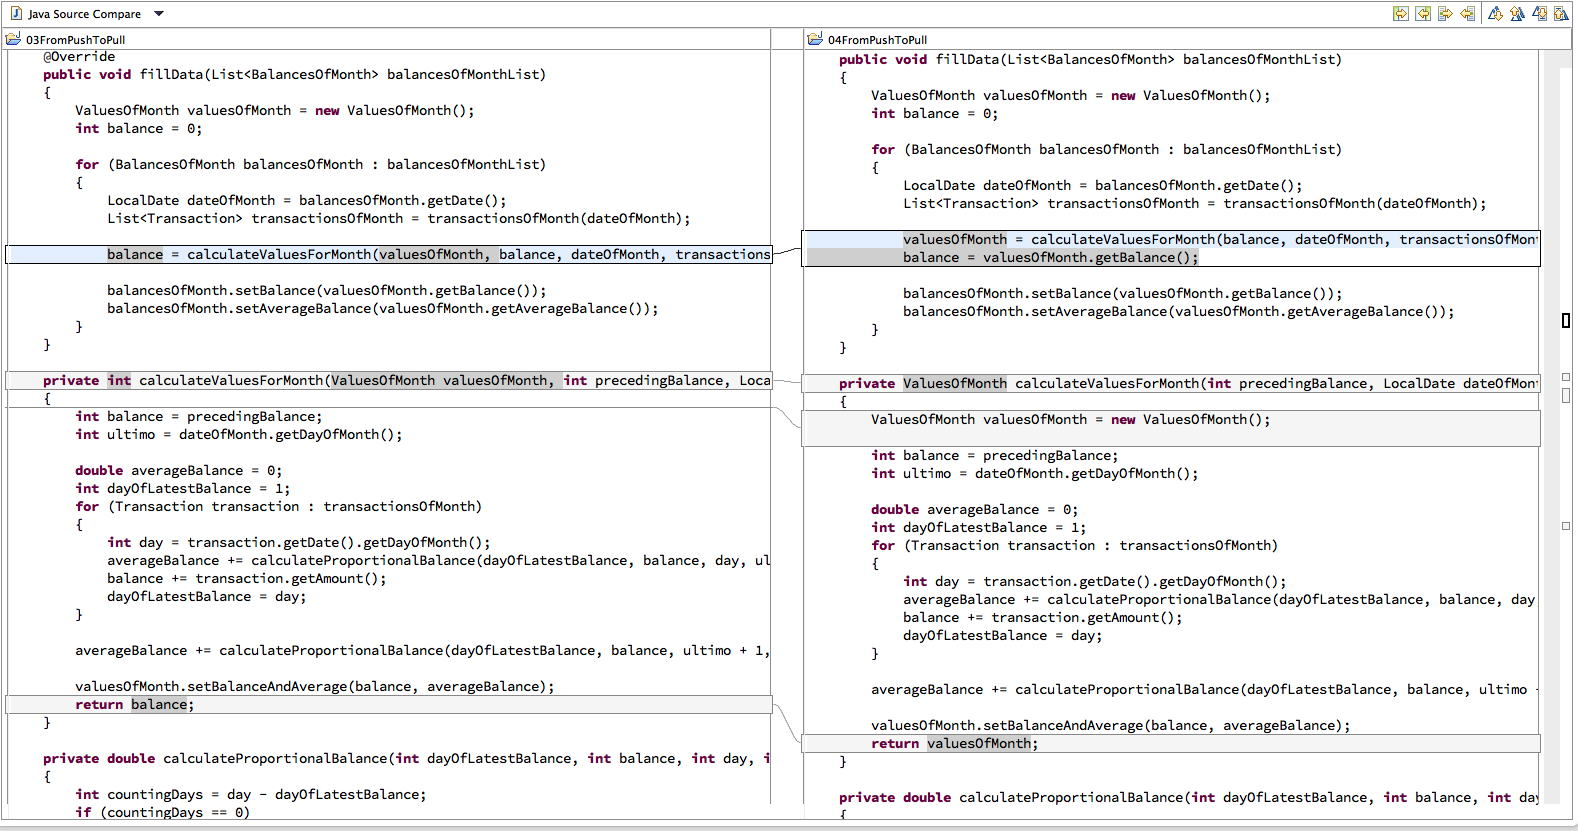
\includegraphics[width=1\textwidth]{CompareViews/03-04.jpg}



\subsection*{Step 05: Separation of concerns (Putting the Code Where it Belongs)}

\subsubsection*{Observations:}
\begin{itemize}
\item The extracted method uses the intermediate data object as in-out-parameter, so it can read values from the previous iteration (if required) and write the calculation results into the data object.
\item The extracted method only operates on this parameter but not on the state of the class it is in. {\em (Code smell: Feature Envy)}
\end{itemize}

\subsubsection*{Solution:}

The extracted calculation method can be moved to the class of the intermediate object. (If this is not done via an automated refactoring: This changes the invocation site of the method as well.)

And don't forget to manually move the method calculateProportionalBalance as well! - After that you can (automatically) change the signature of the extracted method to remove the PushingBalancesCalculator parameter.

\subsubsection*{Modified:}

\texttt{PushingBalancesCalculator.calculateValuesForMonth()} is moved to\\ \texttt{ValuesOfMonth.calculateValues()}

\texttt{PushingBalancesCalculator.calculateProportionalBalance()} is moved to\\ \texttt{ValuesOfMonth.calculateProportionalBalance()}

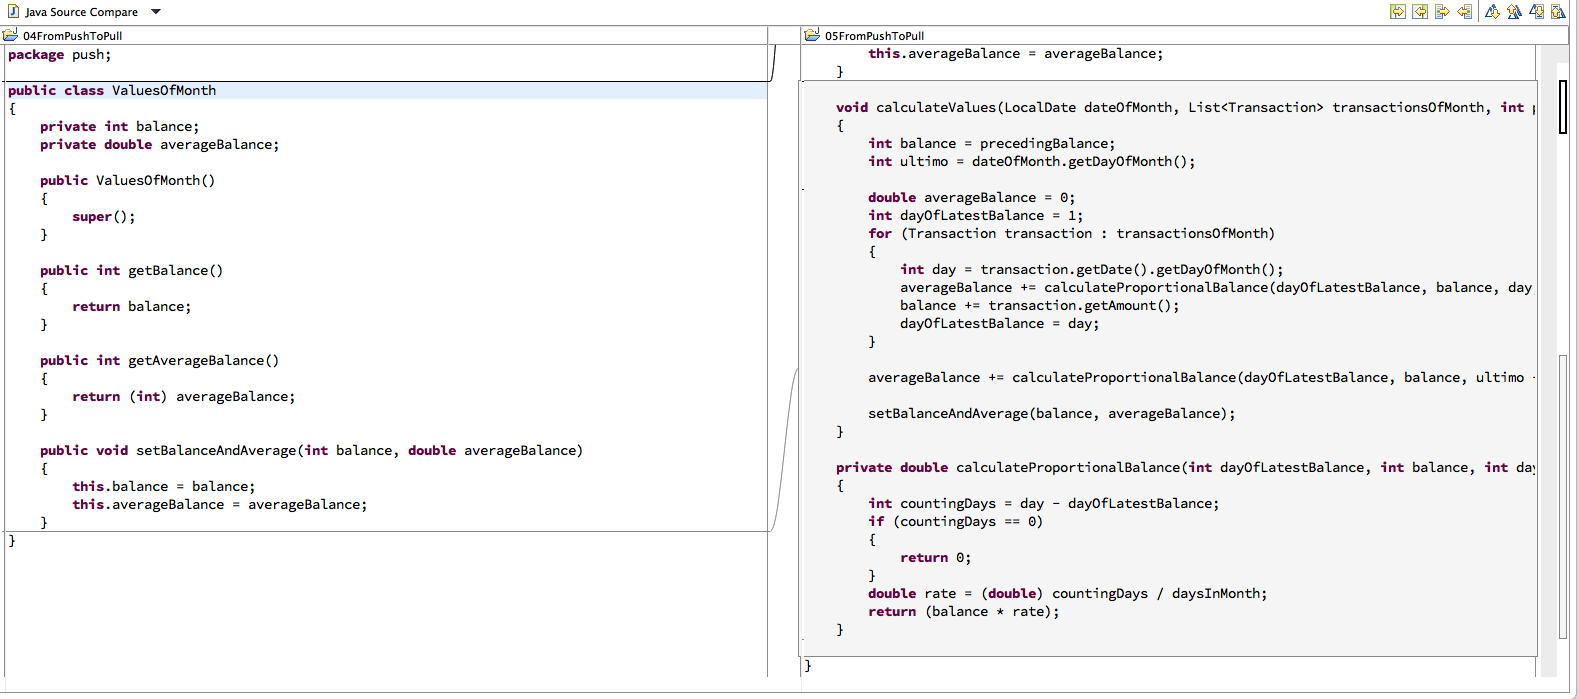
\includegraphics[width=1\textwidth]{CompareViews/04-05-1.jpg}

\texttt{PushingBalancesCalculator.fillData()} (method invocation is adapted to moved method)

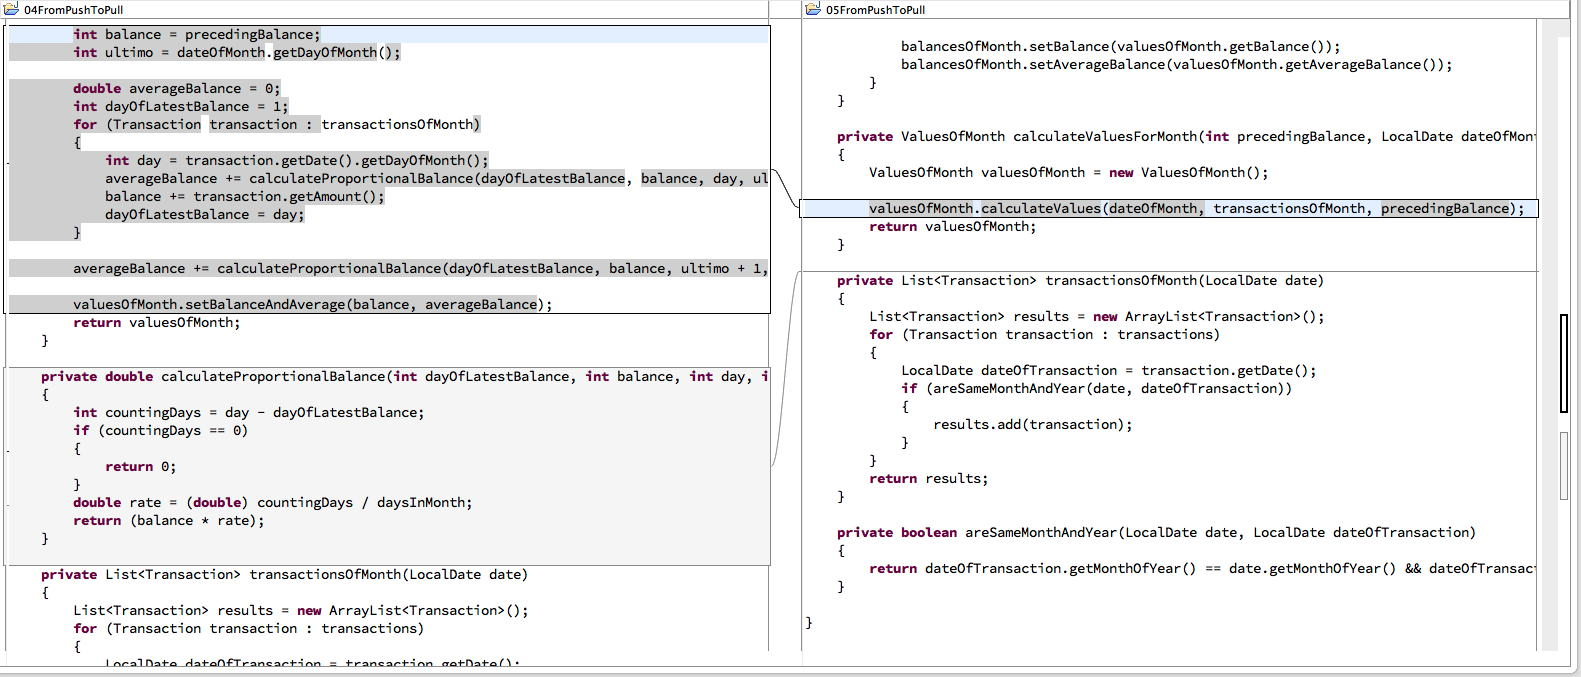
\includegraphics[width=1\textwidth]{CompareViews/04-05-2.jpg}

\subsection*{Step 06: Use New Instance of Intermediate Object for Each Execution of the Inner Loop Body}

\subsubsection*{Observations:}
\begin{itemize}
\item The for loop reuses the same \texttt{ValuesOfMonth} object in each loop iteration.
\item The only value that needs to be transported from one iteration to the next is the balance of the preceding iteration, which is already retrieved anyway.
\end{itemize}

\subsubsection*{Solution:}


In this step, we want each execution of the loop body to create its own intermediate object. If the value calculation uses values from a previous calculation, we need to take care of this and pass on the required values from the previous intermediate object to the calculation method, possibly widening its signature.

In our example, we explicitly pass the preceding balance to the calculation. We have to fetch it from the previous result before creating a new instance.

\subsubsection*{Modified:}

\texttt{PushingBalancesCalculator.fillData()}

\texttt{ValuesOfMonth.calculateValues()}

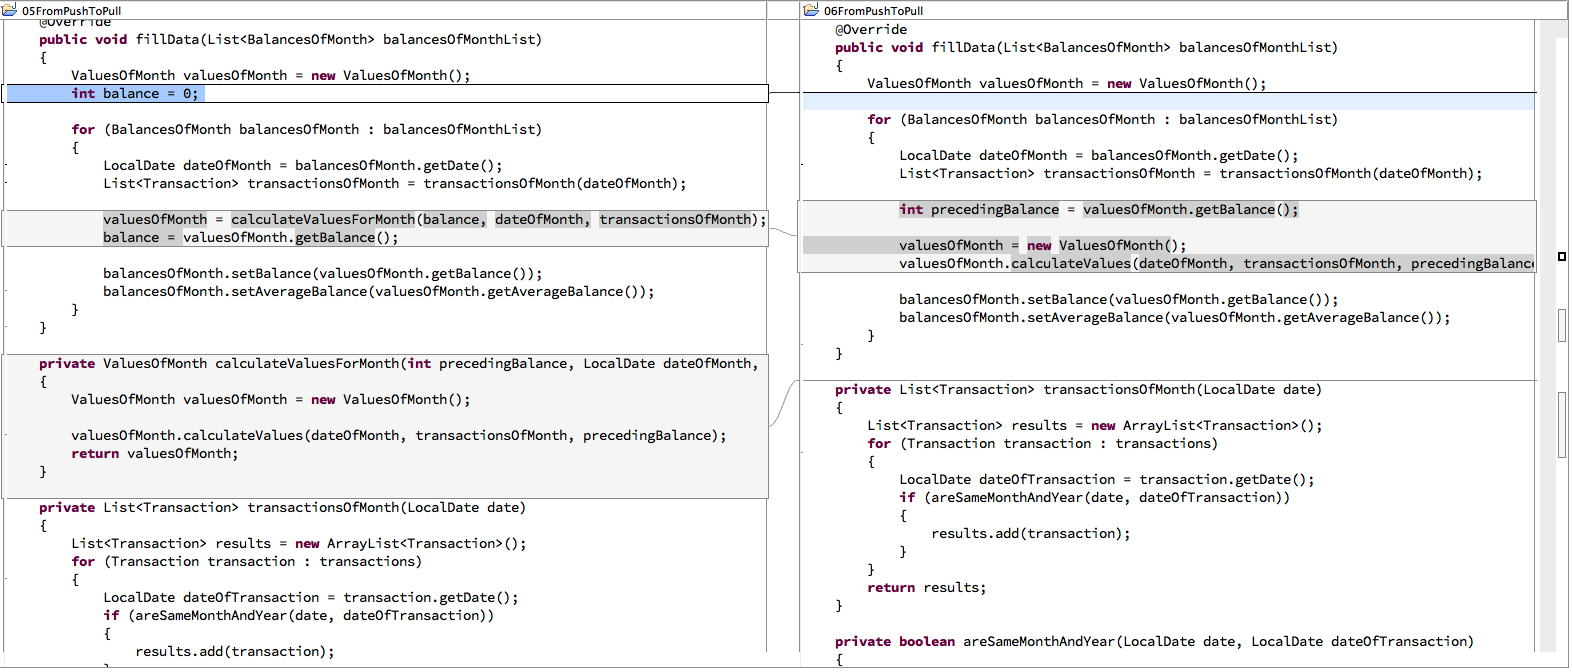
\includegraphics[width=1\textwidth]{CompareViews/05-06.jpg}


\section*{Part III: From Calculating the Values Up-Front to Calculating the Values On-Demand}

\subsubsection*{Overall Goal:}

Currently, all values are calculated up-front with an explicit command from the outside, no matter whether they are needed or not. It would be much nicer if our object could calculate the values on-demand when (and only when) they are needed.

In order to achieve this, we transform the overall calculation method into individual methods that return each value on demand.

\subsection*{Step 07: Remove the Parameters from the Value Calculation Method}

\subsubsection*{Observations:}
\begin{itemize}
\item We still need to explicitly invoke the value calculation on the intermediate object. 
\item We pass all required inputs into the calculation method.
\end{itemize}

\subsubsection*{Solution:}

The first step to removing the calculation method is to pass the input values into the constructor of the result object, thus turning these inputs into state for the calculating object.

\subsubsection*{Modified:}

\texttt{ValuesOfMonth} (fields, constructor, method signature)

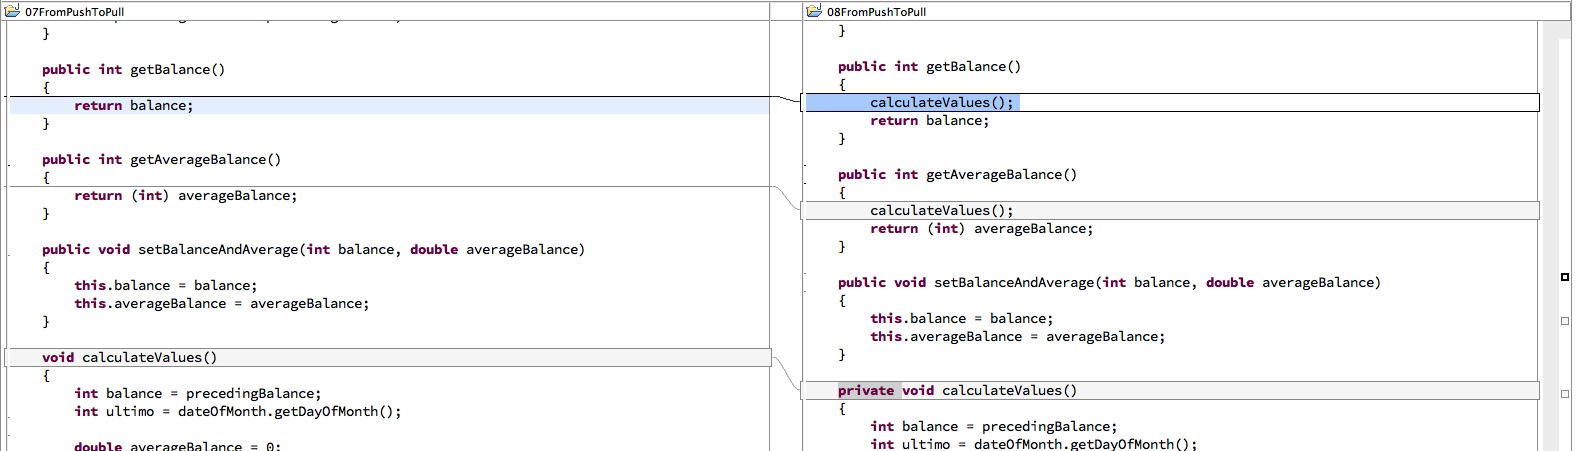
\includegraphics[width=1\textwidth]{CompareViews/06-07-2.jpg}

\texttt{PushingBalancesCalculator} (method and constructor invocation)

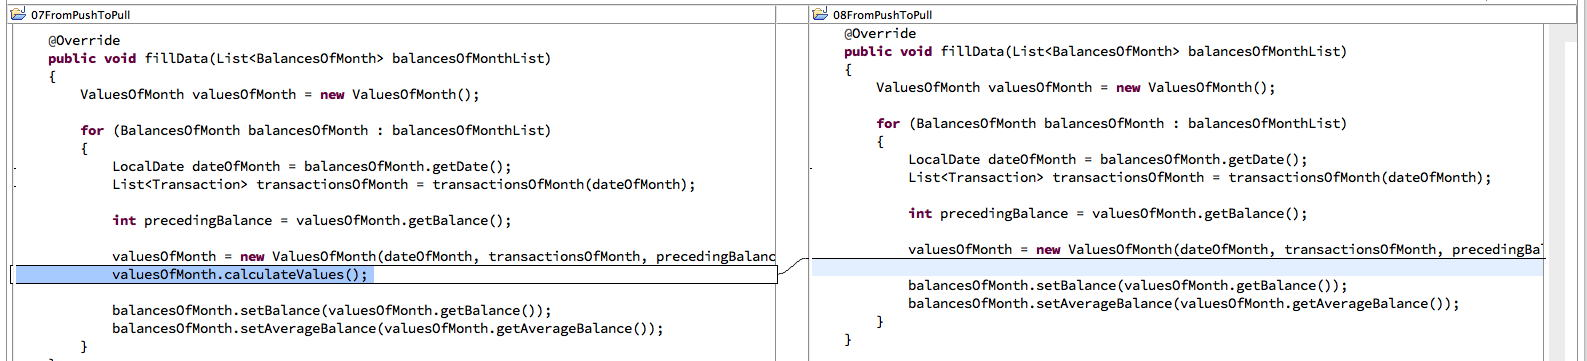
\includegraphics[width=1\textwidth]{CompareViews/06-07-1.jpg}




\subsection*{Step 08: Make the Value Calculation Implicit}

\subsubsection*{Observations:}
\begin{itemize}
\item So far, we still calculate all values at once, in the same method. 
\item This method invokes a setter that writes all values into the intermediate object's attributes in one go (we introduced this setter in Step 1).
\end{itemize}

\subsubsection*{Solution:}
In this step, we move the value calculations to the setters. As a result, \texttt{calculateValues} can be private.

Caution: This is only possible with reentrant (i.~e.~side-effect-free) methods.

\subsubsection*{Modified:}

\texttt{PushingBalancesCalculator.fillData()} (calculation method invocation is removed).

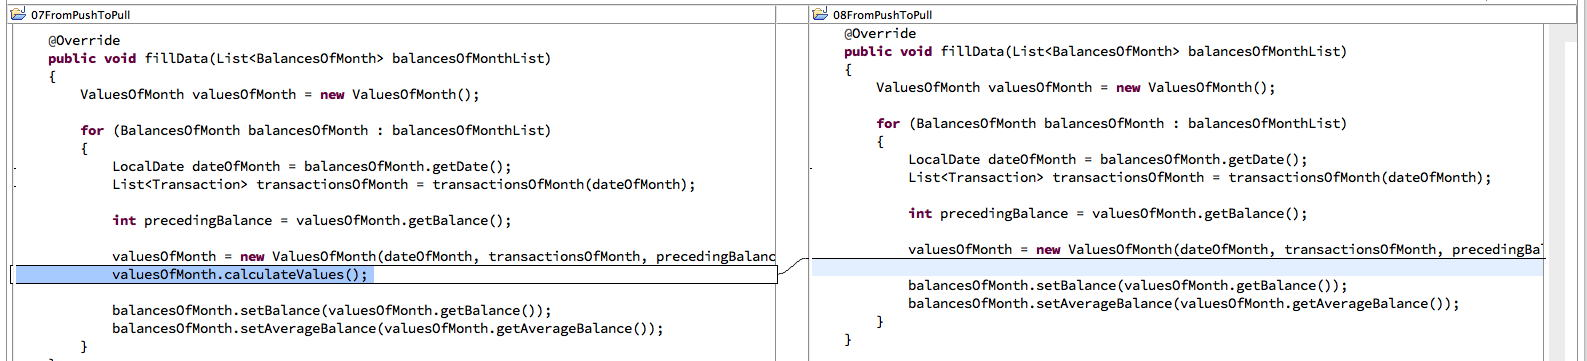
\includegraphics[width=1\textwidth]{CompareViews/07-08-1.jpg}

\texttt{ValuesOfMonth.getBalance()} is modified

\texttt{ValuesOfMonth.getAverageBalance()} is modified


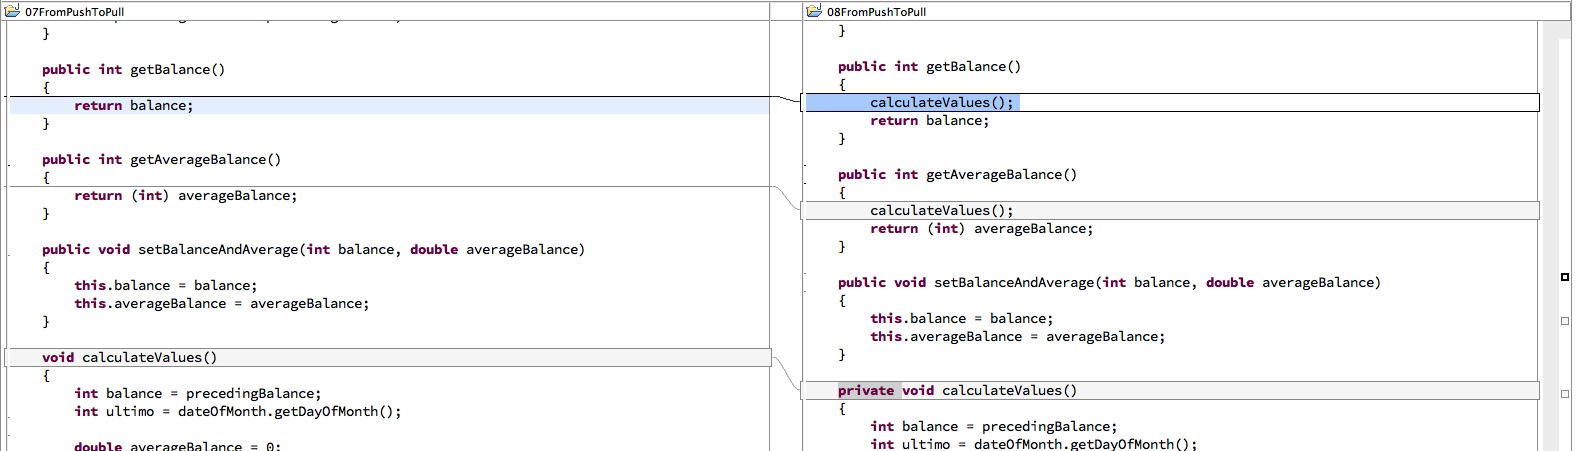
\includegraphics[width=1\textwidth]{CompareViews/07-08-2.jpg}



\subsection*{Step 9: Inline the Value Calculation Method}

\subsubsection*{Observations:}
\begin{itemize}
\item The two getters do the calculations, set the fields and return the values. 
\end{itemize}

\subsubsection*{Solution:}

We can now inline and remove the value calculation method and also the \texttt{setBalanceAndAverage} setter.

Now we can remove all code from each of the getters that is not related to calculating the value for which the getter is responsible. Each of these getters immediately returns the calculated value, without writing it into a field.

Finally, we can remove the fields for balance and averageBalance.

As a result, we have getters for the individual values of the intermediate object which describe exactly how each value is being calculated.

\subsubsection*{Modified:}

\texttt{ValuesOfMonth} (fields, setter and \texttt{calculate...} methods are removed)

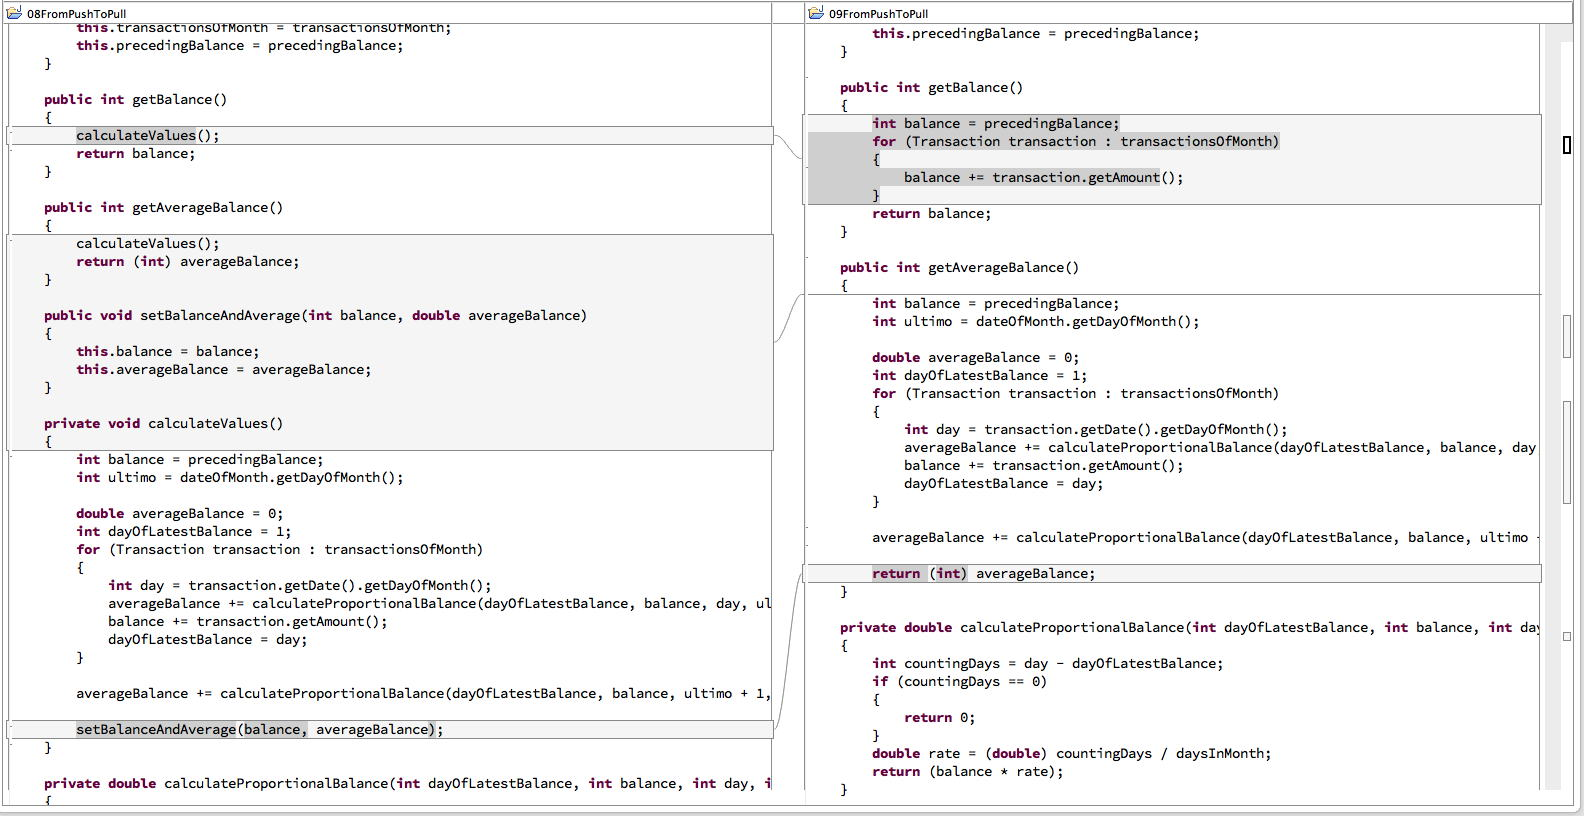
\includegraphics[width=1\textwidth]{CompareViews/08-09.jpg}



\subsection*{Step 10: Simplification}

\subsubsection*{Observations:}
\begin{itemize}
\item The calculation of the average balance is quite complicated.
\item The calculation of the average balance is isolated and easily testable.
\end{itemize}

Now that we can see each value calculation in isolation, we often notice that we can perform simplifications of the algorithms. 

\subsubsection*{Solution:}

We can simplify the algorithm or even rewrite it (with TDD if we like). It is now easy to clarify the business aspects of this logic and to develop a new algorithm. 
\\~

We demonstrate the change of algorithms with an example.
Suppose we have a balance like this:

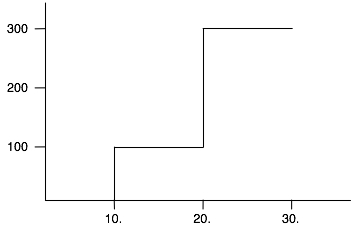
\includegraphics[width=.5\textwidth]{balance.jpg}

i.e.~there is a transaction of 100 on the 10th and a transaction of 200 on the 20th to an initially empty account.
We want to determine the average, which is the area under the graph divided by the number of days in the month.
\\~

The existing algorithm determines the average like this:

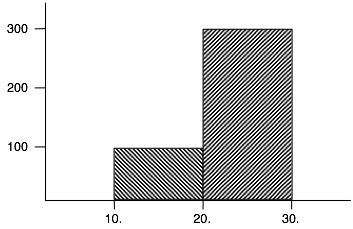
\includegraphics[width=.5\textwidth]{initialAverage.jpg}

Whenever a transaction occurs, the algorithm calculates the area under the graph for the number of days between the previous transaction (or the start of the month) and the current transaction and divides it by the number of days that are between these two dates. The disadvantage is that we have many special cases (beginning and end of month) and that we need to keep track of the current balance and of when the previous transaction happened.
\\~

We prefer to implement the average like this:

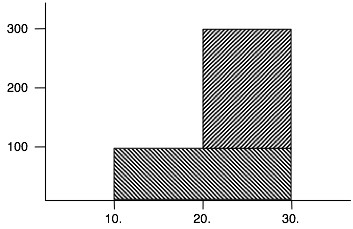
\includegraphics[width=.5\textwidth]{finalAverage.jpg}

Whenever a transaction occurs, this algorithm calculates its average up to the end of the month. This algorithm is much easier to implement because the average of each transaction can be determined in isolation.
\\~

The proof that this algorithm works correctly for transactions with negative amounts is left as an exercise for the reader.

\subsubsection*{Modified:}

\texttt{ValuesOfMonth.getAverageBalance()}

\texttt{ValuesOfMonth.calculateProportionalBalance()} is removed

\texttt{ValuesOfMonth.rateOf()} is created

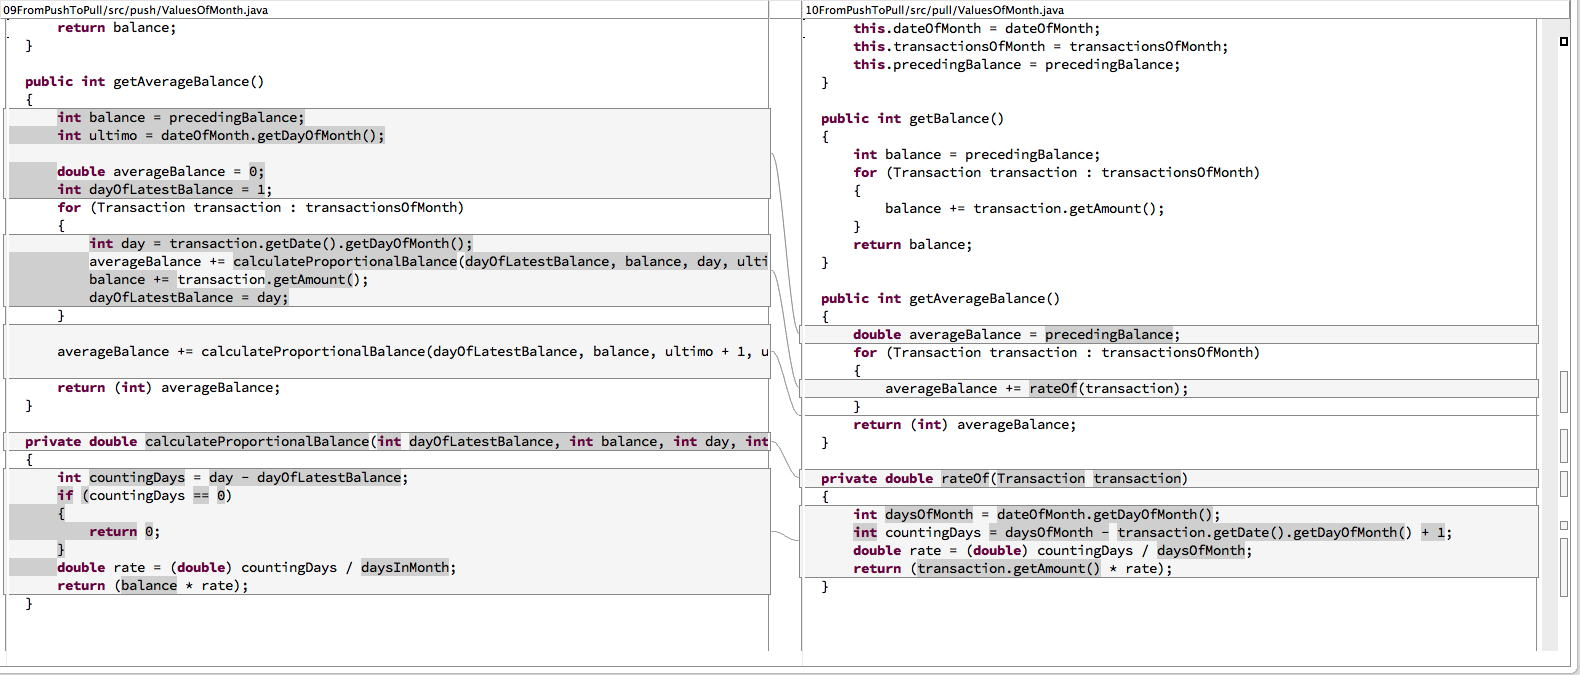
\includegraphics[width=1\textwidth]{CompareViews/09-10.jpg}


\subsection*{Final Step: Achieving the ``Pull'' Structure (Workspace: Pull)}

\subsubsection*{Observations:}

\begin{itemize}
\item The outer for loop from the beginning still uses the same variable for the calculation objects.
\item After one loop iteration, the calculation object is gone. We cannot access the results later on.
\item If we want to access the results again at a later time, we need to recalculate everything again and again.
\end{itemize}

\subsubsection*{Solution:}

Transform the calculation objects into a chained structure of calculation objects (called \texttt{Month}) where each month can access its predecessor's values.

Create this chained structure up-front (using a \texttt{Months}-object). Fill it with all relevant input data.

In the for-loop, simply access the calculated results of the months.

Introduce caching of the calculated results in order to avoid performance issues.

\subsubsection*{Modified:}

\texttt{ValuesOfMonth} gets extended by an interface and variants

\texttt{Months} is extracted from \texttt{PullingBalancesCalculator}

\subsection*{The Final Situation}

\subsubsection*{Observations:}

\begin{itemize}
\item Calculation logic and result structure are now identical
\item We now have intelligent objects instead of stupid data records
\item The algorithms for each value are isolated and clearly visible
\end{itemize}



\end{document}
